\let\negmedspace\undefined
\let\negthickspace\undefined
\documentclass[journal,12pt,onecolumn]{IEEEtran}
\usepackage{cite}
\usepackage{amsmath,amssymb,amsfonts,amsthm}
\usepackage{algorithmic}
\usepackage{graphicx}
\graphicspath{{./figs/}}
\usepackage{textcomp}
\usepackage{xcolor}
\usepackage{txfonts}
\usepackage{listings}
\usepackage{enumitem}
\usepackage{mathtools}
\usepackage{gensymb}
\usepackage{comment}
\usepackage{caption}
\usepackage[breaklinks=true]{hyperref}
\usepackage{tkz-euclide} 
\usepackage{listings}
\usepackage{gvv}                                        
%\def\inputGnumericTable{}                                 
\usepackage[latin1]{inputenc}     
\usepackage{xparse}
\usepackage{color}                                            
\usepackage{array}
\usepackage{longtable}                                       
\usepackage{calc}                                             
\usepackage{multirow}
\usepackage{multicol}
\usepackage{hhline}                                           
\usepackage{ifthen}                                           
\usepackage{lscape}
\usepackage{tabularx}
\usepackage{array}
\usepackage{float}
\newtheorem{theorem}{Theorem}[section]
\newtheorem{problem}{Problem}
\newtheorem{proposition}{Proposition}[section]
\newtheorem{lemma}{Lemma}[section]
\newtheorem{corollary}[theorem]{Corollary}
\newtheorem{example}{Example}[section]
\newtheorem{definition}[problem]{Definition}
\newcommand{\BEQA}{\begin{eqnarray}}
\newcommand{\EEQA}{\end{eqnarray}}
\newcommand{\define}{\stackrel{\triangle}{=}}
\theoremstyle{remark}
\newtheorem{rem}{Remark}

\begin{document}

\title{9.2.19}
\author{ee25btech11056 - Suraj.N}
\maketitle
\renewcommand{\thefigure}{\theenumi}
\renewcommand{\thetable}{\theenumi}

\begin{document}

\textbf{Question :} Find the area of the smaller part of the circle \(x^{2}+y^{2}=a^{2}\) cut off by the line \(x=\frac{a}{\sqrt{2}}.\)

\textbf{Solution :}

\begin{table}[h!]
  \centering
  \begin{tabular}{|c|c|}
\hline
\textbf{Name} & \textbf{Value} \\
\hline
Circle & $\vec{x}^\top\vec{x} - a^2 = 0$ \\
\hline
Line & $\vec{x} = \myvec{\tfrac{a}{\sqrt{2}} \\ 0} + \kappa\myvec{0 \\ 1}$ \\
\hline
\end{tabular}

  \caption*{Table : Circle}
  \label{9.2.19}
\end{table}

The parameters for the circle are :

\begin{align}
  \vec{V} &= \vec{I} & \vec{u} &= \vec{0} & f &= -a^2 
\end{align}

The parameters for the line are :

\begin{align}
  \vec{h} &= \myvec{\tfrac{a}{\sqrt{2}}\\0} & \vec{m} &= \myvec{0\\1}
\end{align}

Substituting these in the below equation to find the intersection points :

\begin{align}
\kappa_i
  &= \frac{1}{\vec{m}^\top \vec{V}\vec{m}}
     \left(
       -\,\vec{m}^\top\big(\vec{V}\vec{h}+\vec{u}\big)
       \;\pm\;
       \sqrt{ \big[\vec{m}^\top(\vec{V}\vec{h}+\vec{u})\big]^2
       - g(\vec{h})\,\big(\vec{m}^\top \vec{V}\vec{m}\big)}
     \right)\\
    g(\vec{x}) &= \vec{x}^\top\vec{x} - a^2 \\
    g(\vec{h}) &= \vec{h}^\top\vec{h} - a^2 \\
\kappa_i &=\left(
       -\,\vec{m}^\top\vec{h}
       \;\pm\;
       \sqrt{a^2 -\vec{h}^\top\vec{h}}
     \right)\\
  \kappa_i &= \frac{a}{\sqrt{2}},-\frac{a}{\sqrt{2}}
\end{align}

Therefore the points of intersection are :

\begin{align}
  \vec{P_1} &= \myvec{\tfrac{a}{\sqrt{2}}\\\tfrac{a}{\sqrt{2}}} & \vec{P_2} &= \myvec{\tfrac{a}{\sqrt{2}}\\-\tfrac{a}{\sqrt{2}}}
\end{align}

Thus the area of the smaller part of the circle cut off by the line is :

\begin{align}
  2 \int\limits_{\frac{a}{\sqrt{2}}}^{a}\! \sqrt{a^2 - x^2}\, dx &= \frac{a^2}{2}\left(\frac{\pi}{2} - 1\right)
\end{align}

\pagebreak

\begin{figure}[h!]
  \centering
  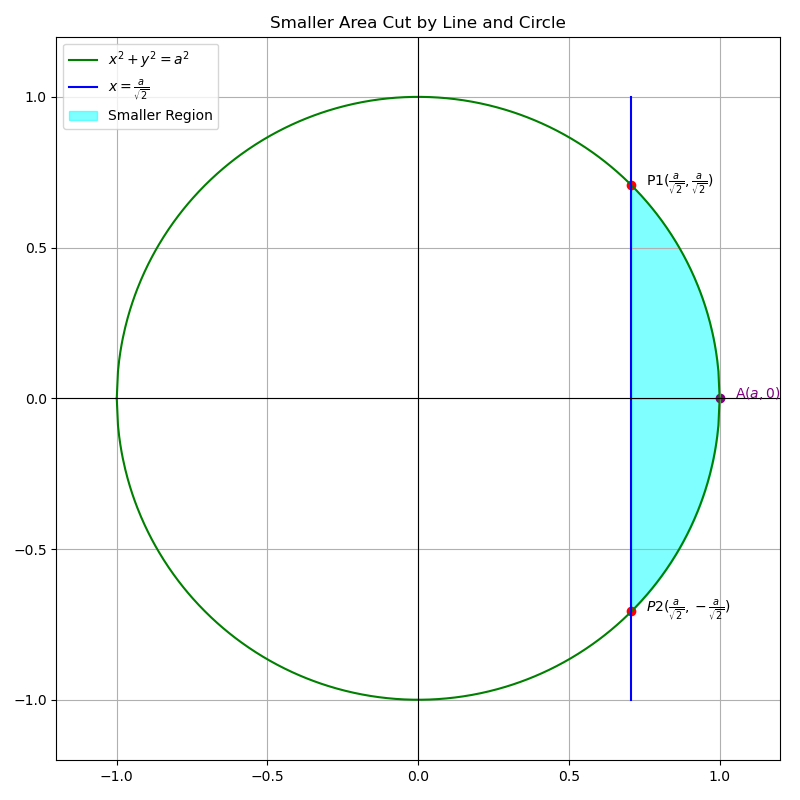
\includegraphics[width=0.7\columnwidth]{figs/circle_area.png} 
   \caption*{Fig : Circle}
  \label{Fig1}
\end{figure}

\end{document}
